\chapter{Sobre la empresa}

	\section{Historia de Movalsys S.L}
		Movalsys es una empresa que se constituye en diciembre de 2015 y que surge de la experiencia investigadora de dos grupos de investigación (Álgebra y Aplicaciones y Biomecánica y Fisiología del movimiento (BIOFIM)) de la Universidad Pública de Navarra. 
		
		Movalsys S.L. desarrolla y comercializa tecnología para la medición rápida y sencilla de los parámetros biomecánicos que caracterizan el movimiento humano. Esta tecnología no se limita a la mera obtención de dichos parámetros, sino que se apoya en el conocimiento reunido durante diez años por investigadores de Universidad Pública de Navarra para contextualizarlos y ofrecer una
		interpretación simple y directa del estado físico del sujeto y de su rendimiento.
		El objetivo de Movalsys es ofrecer a los profesionales de la salud herramientas que les sirvan de apoyo en el diagnóstico, el seguimiento y la óptima recuperación de sus pacientes, facilitándoles el acceso a la valoración biomecánica del movimiento humano.
	
	
	\section{Dedicación de la empresa}
	 
	Este equipo multidisciplinar lleva ocho años realizando investigaciones sobre el análisis de señales biomecánicas proporcionadas por sensores inerciales y sus avances han sido publicados en importantes revistas científicas en Fisioterapia, Geriatría, Ingeniería y Matemáticas.
	
	La dedicación de la empresa consiste fundamentalmente en la obtención y procesado de parámetros mediante sensores inerciales, es decir, en el análisis del movimiento. Por tanto su campo de aplicación puede ser tanto la práctica deportiva (mejora de rendimiento, prevención de lesiones), como el de la rehabilitación (riesgo de caídas, fragilidad,etc.). Actualmente se está explorando el campo de la neuro-rehabilitación y de la prevención de riesgos laborales en las industrias (ver figura \ref{mercado}). 
	 \begin{figure}[H]
	 	\centering
	 	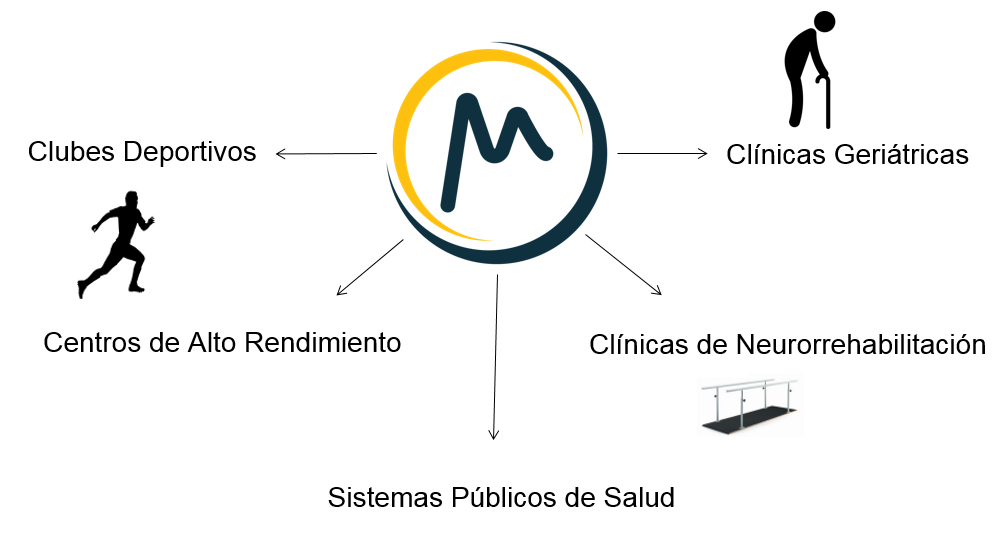
\includegraphics[width=0.8\textwidth]{./graphics/mercado}\label{mercado}
	 	
	 \end{figure}
	\section{Estructura de la empresa} \label{empresa}
	

		Movalsys S.L. es una sociedad limitada en la que todos sus trabajadores son socios de la misma y además cuentan con colaboración externa para el desarrollo de su actividad.
		
		A continuación se describen los roles de cada uno de los mismos:
		\begin{itemize}
			\item \textbf{Mariano Velasco}: Director gerente. Su objetivo es principalmente el de reunirse con miembros de otras empresas para conseguir proyectos. Es la imagen pública de la empresa. Su dedicación es principalmente la de la gestión de la empresa. Se encarga tanto de la coordinación del equipo como de la burocracia. Además, es el principal encargado de reunirse con diferentes clientes así como de realizar la promoción de la empresa en diferentes eventos.
			 \begin{figure}[H]
			 	\centering
			 	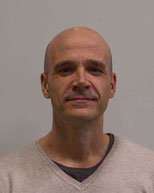
\includegraphics[width=0.25\textwidth]{./graphics/mariano}

			 \end{figure}
			\item \textbf{Pablo Lecumberri}: Es el ingeniero de software, encargado del software de medición que utiliza la empresa. Se trata de un empleado de carácter técnico que resulta fundamental especialmente en las reuniones con clientes.
			\begin{figure}[H]
				\centering
				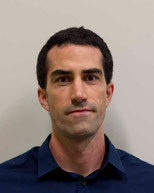
\includegraphics[width=0.25\textwidth]{./graphics/pablo}
				
			\end{figure}
			\item \textbf{Marisol Gómez}: directora de investigación. Se encarga de la búsqueda de ayudas de investigación y de buscar nuevas áreas de desarrollo de la empresa. Actualmente su actividad está centrada en la neuro-rehabilitación.
			\begin{figure}[H]
				\centering
				
\includegraphics[width=0.25\textwidth]{./graphics/marisol}
				
			\end{figure}
			\item \textbf{Alicia Martínez}: Responsable de ventas. Se encarga de la gestión de facturas así como de la búsqueda de nuevos clientes. 
			\begin{figure}[H]
				\centering
				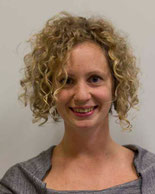
\includegraphics[width=0.25\textwidth]{./graphics/alicia}
				
			\end{figure}
			\item \textbf{Nora Millor}: Responsable de atención al cliente. Es al encargada de estar en contacto con clientes, realizar un seguimiento de funcionamiento del sistema y de 
			\begin{figure}[H]
				\centering
				
\includegraphics[width=0.25\textwidth]{./graphics/nora}
				
			\end{figure}
			\item \textbf{Mikel Izquierdo}: es catedrático y director del departamento de Ciencias de la Salud. Se trata de un profesional muy reconocido en el campo de la salud y por ello también actúa como asesor y se dedica además a la búsqueda de contactos, lo cual en esta etapa de la empresa resulta imprescindible.
			\begin{figure}[H]
				\centering
				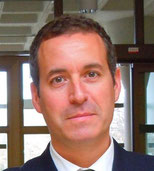
\includegraphics[width=0.25\textwidth]{./graphics/mikel}
				
			\end{figure}
			\item \textbf{Igor Setuain}: colaborador externo. Es doctor en fisioterapia y asesora a la empresa sobre los parámetros obtenidos en las mediciones dándoles sentido clínico.
			
		\end{itemize}
		
	Además de sus funciones principales, Pablo, Marisol, Nora, Alicia y Mariano se encargan de hacer el análisis de señales y de las mediciones. No participan todos siempre puesto que depende de la carga de trabajo de cada uno.
	
	Con respecto a la jerarquía de la empresa puede decirse que es plana, es decir, a pesar de existir la figura de director gerente, las decisiones se realizan de forma que todos los socios participan en ella. Se discuten en las reuniones semanales. El hecho de que cada empleado sienta responsabilidad en la toma de decisiones hace que se sientan integrados y valorados en la empresa, por tanto, que crezca su motivación y, además obtener diferentes perspectivas sobre un tema que permiten que las decisiones se enriquezcan. Además el hecho de que sean socios de la empresa provoca un sentimiento de responsabilidad en la misma, ya que la empresa es suya.
		


	\section{Plan estratégico}
	
	El plan estratégico es un programa de actuación que consiste en aclarar lo que pretendemos conseguir y cómo nos proponemos conseguirlo. Debido a que se trata de una start-up, no existe un plan estratégico claro ya que precisamente lo que caracteriza a este tipo de empresas es que se encuentran en fase de búsqueda de un modelo de negocio beneficioso para ellas.
		
		Actualmente uno de los trabajos que se desarrollan en la empresa es la búsqueda de producto y clientes/proyectos y mediante dicho trabajo se pretende buscar una solución para el plan estratégico de la empresa. Las decisiones se toman según aparezcan clientes, pero la definición clara de cómo actuar ante ciertas propuestas o qué productos ofrecer no está cerrada del todo debido a que todavía es necesaria la evaluación de las posibilidades que ofrece la empresa y cuáles de estas resultan más beneficiosas.
		
		
	
	\section{Funcionamiento general}
	
	El funcionamiento de la empresa es simple debido al reducido tamaño de la misma (5 empleados + 1 becaria). Cada uno de los componentes tiene claro el rol que desempeña en la empresa.
	
	La semana se compone generalmente de reuniones con clientes para buscar nuevos proyectos y de desarrollar aquellos que están en marcha, es decir, realizar análisis de los datos medidos y los informes oportunos. Además cada miembro desarrolla en paralelo cada una de las funciones de la cual es responsable (apartado \ref{empresa}).
	
	Debido al buen ambiente de trabajo ya que se conocen desde hace varios años, la motivación es alta. Además, a esto se le suma el que los miembros son socios por lo que tienen una motivación adicional por que todo salga bien. 
	
	Con respecto a retención de personal, están interesados en que llegue el día en el que puedan contratar a gente para repartir carga de trabajo. En mi caso, han estado enseñándome continuamente lo que hacen en la empresa y me han enseñado a realizar algunos de los análisis que llevan a cabo. Además, cuentan conmigo para un proyecto futuro relacionado con la temática de mi Trabajo Fin de Máster. Están dispuestos a dar oportunidad a gente nueva y a que la empresa crezca. Han ido guiando mi participación en las actividades con mucho interés e intentando integrar mi trabajo en el día a día de la empresa lo que ha hecho que mi interés y motivación en la empresa crezcan.
	
	